Variabilita srdeční frekvence (\gls{HRV}) vypovídá o časové variabilitě mezi
jednotlivými srdečními stahy a umožňuje nahlédnout do regulace různých tělesných
funkcí autonomním nervovým systémem. Následující kapitola se zabývá způsoby
jakými je možné takové nahlédnutí realizovat a zároveň poukazuje na současné
nedostatky této problematiky, které je třeba brát v potaz. Nejdříve je ale na
místě uvést obecné objasnění vzniku a souvislosti variability srdeční frekvence
s funkcionalitou srdce. Regulační pochody autonomního nervového systému spojené
s \gls{HRV} byly popsány v minulé kapitole (zjednodušeně viz
Obr.~\ref{fig:hrv_diagram}D).

\begin{figure}[h]
    \begin{center}
        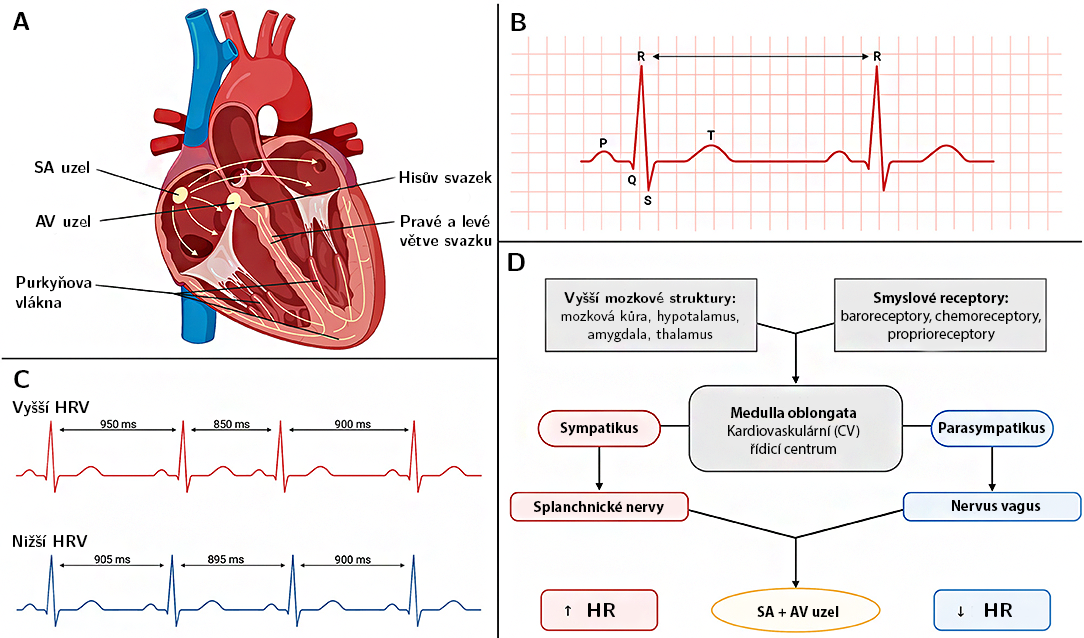
\includegraphics[width=1\linewidth]{figures/hrv_diagram}
        \caption{\textbf{(A)} Převodní systém srdeční; \textbf{(B)} Schéma
            \gls{EKG} záznamu elektrické aktivity; \textbf{(C)} Vysoká vs. nízká
            variabilita srdeční frekvence; \textbf{(D)} Schéma znázorňující
            různé faktory ovlivňující \gls{HR} a \gls{HRV} resp. zjednodušená
            část \gls{NVI} modelu (Upraveno a převzato z~\cite{Lujan2021})}
        \label{fig:hrv_diagram}
    \end{center}
\end{figure}

Jak již bylo řečeno, \gls{HRV} lze získat jako časovou diferenci mezi jednotlivými
srdečními údery, přičemž úder označujeme jako depolarizaci komor. To je část
srdečního cyklu, během které dochází ke genezi QRS komplexu. Aby bylo možné tuto
časovou diferenci vypočítat, je potřeba zmíněný komplex detekovat. K tomu se
využívá elektrokardiogram neboli záznam elektrické aktivity srdce, na kterém QRS
komplex představuje vývoj elektrické aktivace komor myokardu. Srdeční cyklus a
anatomie srdce již byly detailně popsány v~\cite{Stejfa2006,Weinhaus2005,Cihak2016}.
EKG záznam společně s QRS komplexem lze vidět na ilustraci~\ref{fig:hrv_diagram}B.

K detekci QRS komplexu se primárně využívá jeho pozitivní kmit neboli R vlna,
která se v \gls{EKG} signálu za fyziologických podmínek vyskytuje periodicky, v
závislosti na srdečním rytmu, konkrétně na autorytmických buňkách. Tyto srdeční
buňky generují stimulační elektrické potenciály, jež iniciují srdeční stah.
Hlavnimi dvěma iniciátory (pacemakerami), určující srdeční frekvenci, jsou
sinoatriální (\gls{SA}) a atrioventrikulární (\gls{AV}) uzel. Převodní systém
srdeční byl již podrobně popsán v~\cite{Stejfa2006,Weinhaus2005,Goldberger2017}
a lze vidět na Obr.~\ref{fig:hrv_diagram}A. Za účelem detekce samotné se využívá
mnoho algoritmů založených například na: vlnkové nebo Hilbertově transformaci,
prahování nebo neuronových sítích. Každý algoritmus zároveň samozřejmě využívá a
těží ze svého vlastního způsobu předzpracování EKG. Některé populární algoritmy
popsali Porr a Howell v~\cite{Porr2019}. Fluktuaci časových diferencí mezi po
sobě jdoucími R vlny a náležitou změnu HRV lze pozorovat na
Obr.~\ref{fig:hrv_diagram}C.

\subsection{Trendy v analýze HRV}
\label{subsec:hrv_analysis_trends}
Oblast vývoje problematiky analýzy variability srdečního rytmu je možné rozdělit
na několik podskupin. První podskupinu tvoří příznaky použité k analýze. Výběr
\gls{HRV} příznaků (parametrů) hraje významnou roli v rámci mapování vnějších
vlivů na funkci biosignálu. Z počátku se využívalo pouze deskriptivní statistiky
na řady nasbíraných hodnot srdečního rytmu pro účely odhalení srdečních
patologií. Zlom ale nastal v 70. letech 20. století, kdy se k analýze začaly
využívat R--R intervaly, a došlo tak k vývoji nových časových parametrů,
například \gls{RMSSD}, pNN50 nebo SDNN, které se stále hojně využívají. Poté
přišla na řadu spektrální a nelineární analýza, tedy frekvenční a nelineární
parametry, které sebou přinesli i nový vizuální nadhled. V poslední době se
používá hlavně časovo-frekvenční analýza, během které se aplikují spektrální
metody na specificky dlouhá časová okna a získají se tak frekvenční parametry
jako LF (Low Frequency) nebo HF (High Frequency). Je tak umožněno sledování
okamžitých změn \gls{HRV}, což může účinně diagnostikovat například
kardiovaskulární onemocnění~\cite{Shaffer2014,Ishaque2021}.

\begin{table}[h!]
    % \setlength{\tabcolsep}{10pt}
    \renewcommand{\arraystretch}{1.2}
    \scriptsize
    \centering
    \begin{threeparttable}
        \caption{Vybrané parametry z časové a frekvenční oblasti~\cite{Ishaque2021}}
        \label{tab:hrv_params}
        \begin{tabular}{p{2cm}p{12cm}}
            \toprule
            Parametr & Popis                                                                                                                                                        \\ \midrule
            SDNN     & Směrodatná odchylka intervalu mezi dvěma normálními srdečními tepy (NN). NN měří celkový výkon. Snižuje se v reakci na \gls{CL}                              \\
            RMSSD    & Střední kvadratická hodnota po sobě jdoucích rozdílů mezi normálními srdečními tepy. Primárně se řídí aktivitou \gls{PNS}                                    \\
            pNN50    & Vyjadřuje procento rozdílu spojeného s intervalem NN, který se liší o více než 50 ms. Korelaci s aktivitou \gls{PNS}, RMSSD, HF                              \\
            SD1      & Nelineární proměnné odvozené z Poincarého grafu. Sdílí vysokou korelaci s HF, RMSSD. Snižuje se v důsledku \gls{CL}                                          \\
            SD2      & Nelineární proměnné odvozené z Poincarého grafu. Sdílí vysokou korelaci s LF. Zvyšuje se v reakci na \gls{CL}                                                \\
            GSR std  & Směrodatná odchylka spojená s elektrodermální aktivitou. Zvyšuje se během \gls{CL}                                                                           \\
            GSR mean & Průměrná hodnota získaná měřením rychlosti změn spojených s aktivitou EDA. Zvyšuje se během \gls{CL}                                                         \\
            RSP rate & Představuje frekvenci dýchání, zvýšení respirační frekvence vede ke zvýšení aktivity \gls{PNS}, VF a snížení LF a aktivity SNS. Zvýšení v reakci na \gls{CL} \\
            LF       & Reprezentuje 0,04--0,15 Hz v rámci PSD\tnote{1} ~a většinou se používá k označení aktivity \gls{SNS} ale může specifikovat i aktivitu \gls{PNS}              \\
            HF       & Představuje frekvenční rozsah 0,15--0,40 Hz a označuje výhradně aktivitu \gls{PNS}                                                                           \\ \bottomrule
        \end{tabular}
        \begin{tablenotes}
            \item [1] Výkonová spektrální hustota (anglicky Power Spectral
            Density) --- vyjadřuje výkon obsažený v určitém intervalu spojitého
            frekvenčního spektra
        \end{tablenotes}
    \end{threeparttable}
\end{table}

Do další podskupiny lze zařadit způsoby měření \gls{HRV}. Od 90. let 20. století
se výzkum \gls{HRV} rozšířil o analýzu využitím krevního tlaku a dýchání
prostřednictvím fotopletysmografie (\gls{PPG}) a hrudních pásů. Došlo tak k
prohloubení HRV výzkumu vzhledem k multimodálnímu přístupu měření. Od roku 2000
se využitím dvanáctisvodového EKG začali v klinické praxi efektivněji analyzovat
srdeční patologie. Současně se využívá nositelných technologií (tzv. wearables)
v podobě například hodinek na zápěstí, které však často měřené parametry
poskytují pouze agregovaně za určité časové úseky. Výhodou je sice jejich
mobilita ale na úkor přesnosti poskytovaných dat. Detailní popis zmíněných
podskupin společně s dalšími trendy byl již uveden v~\cite{Ishaque2021}.

\subsection{Struktura HRV indexů}
\label{subsec:hrv_indices}
Vzhledem k popularitě analýzy \gls{HRV} napříč obory vznikla problematika
týkající se interpretace dostupných metrik. Jedním z hlavních problémů je tedy
nedostatečné pochopení funkčního vztahu mezi \gls{HRV} ukazateli a
fyziologickými procesy. Také se tyto ukazatele často používají zaměnitelně, což
jen přispívá k nejasnostem ohledně jejich skutečného významu
(funkce)~\cite{Fatisson2016,hayano2019}. Zároveň se často \gls{HRV} metriky
používají kombinovaně. To představuje několik problémů při interpretaci výsledků
výzkumu a může být příčinou nekonzistentních výsledků. Dalším problémem je
reprodukovatelnost, jelikož různé studie zkoumající stejný jev mohou při popisu
vztahu s variabilitou srdeční frekvence vycházet z různých ukazatelů. Také se
často nebere ohled na podobnost a překrývání mnoha těchto ukazatelů. Studie
například ukázaly, že indexy v časové a frekvenční oblasti, jako je RMSSD a
pNN50, spolu silně korelují a jsou vysoce spojeny s výkonem HF. V důsledku toho
lze tyto míry považovat za zaměnitelné při hodnocení parasympatické modulace
\gls{HRV}. Nejasnosti ohledně fyziologických důsledků těchto ukazatelů zvyšují
právě náročnost objasnění jejich
výsledků~\cite{Bigger1989,Rohila2020,Malik1996,Ishaque2021}.

Je také třeba poznamenat, že výpočet RMSSD zahrnuje výpočet rozdílů mezi po sobě
jdoucími R--R (N--N) intervaly. V důsledku toho tento index odráží především
vysokofrekvenční oscilační vzorce srdečního rytmu a není ovlivněn dlouhodobými
změnami. Naproti tomu SDNN, o němž se předpokládá, že zachycuje jak sympatickou,
tak parasympatickou aktivitu, je silně spojen s celkovým výkonem ve výkonovém
spektru \gls{HRV}~\cite{Bigger1989,Malik1996,Ishaque2021,Acharya2006}.

V posledních letech se parametry SD1 a SD2 konvenčně interpretují jako
nelineární. Toto tvrzeni bylo však znehodnoceno matematickým důkazem, který
potvrdil, že metriky RMSSD a SD1 jsou ekvivalentní. Tím pádem studie, které
uvádějí tyto dva krátkodobé \gls{HRV} indexy často vágně dospívají k podobným
statistickým výsledkům, aniž by tuto ekvivalenci
rozpoznaly~\cite{Ciccone2017,Tam2021,Leite2015,Rohila2020,Peng2015}.

Některé studie navíc zaznamenaly podobnosti mezi poměrovými parametry SD1/SD2 a
LF/HF při hodnocení rovnováhy mezi krátkodobou a dlouhodobou variabilitou
srdečního rytmu. Nezohlednění těchto překryvů v analýzách může vést ke
statistickým chybám. Ty mohou zahrnovat přílišnou důvěru v závěry (projevující
se falešně vysokým počtem parametrů shodujících se s určitým trendem), problémy
s kolinearitou (pokud je jako prediktory použito více metrik současně),
potenciální nadměrnou korekci (např. prostřednictvím metod úpravy p-hodnoty
Bonferroniho typu) a zbytečnou složitost
výsledků~\cite{Tam2021,Rohila2020,Dormman2013,Guzik2013,Brennan2002}.
